\chapter{Weryfikacja}
\label{chapter:verify}

Weryfikacja działania platformy odbyła się na podstawie uruchomienia na niej historycznych programów studentów.
Wykorzystane aplikacje zostały utworzone w ramach przedmiotu ”Podstawy Programowania” w semestrze zima 2018.

Proces weryfikacji można podzielić na następujące kroki:
\begin{enumerate}
    \item Przeanalizowanie zadania projektowego i dostępnych aplikacji studenckich.
    \item Lokalne uruchomienie programów.
    \item Zdefiniowanie nowego projektu na platformie wraz z przypadkami testowymi.
    \item Uruchomienie aplikacji studentów z poprzednich lat na platformie i przedstawienie otrzymanych wyników.
    \item Podsumowanie.
\end{enumerate}

Przebieg powyższych kroków został opisany w kolejnych podrozdziałach.


\section{Analiza zadania projektowego}
\label{analysis_students_projects}

W celu weryfikacji platformy posłużono się kodem studentów napisanym w ramach przedmiotu podstawy programowania.
Zadaniem studentów było napisanie programu odzwierciedlającego logikę gry planszowej ”Hey, that’s mine fish”.
Aplikacja miała umożliwiać interaktywny oraz autonomiczny rodzaj rozgrywki.
Zadaniem programów było wczytanie wejściowego układu planszy z pliku, wykonanie zadanej akcji oraz zapisanie zmodyfikowanego układu planszy do pliku.
Format pliku jest jednoznacznie określony w~treści zadania i składa się z:
\begin{itemize}
    \item \textit{Wiersz 1}: \textit{m n} - dwóch wartości liczbowych oznaczających rozmiar planszy.
    \item \textit{Wiersze od 2 do m+1}: \textit{n} pól odseparowanych znakiem spacji, każde z pól jest definiowane przez dwie cyfry.
    Pierwszą oznaczającą liczbę ryb na danym polu (od 0 do 3) oraz druga będącą identyfikatorem gracza znajdującego się obecnie na tym polu (od 1 do 9 lub 0 jeśli pole nie jest zajęte).
    \item \textit{Wiersze od m+2}: trzech pól, reprezentujących kolejno: nazwę gracza (String), identyfikator gracza (od 1 do 9), liczbę punktów uzyskanych przez gracza.
\end{itemize}

Zgodnie z założeniami programy mają przyjmować następujące parametry:
\begin{itemize}
    \item \textit{phase=phase\_mark}, parametr \textit{phase\_mark} może przyjąć jedną z dwóch wartości: \textit{placement} (rozmieszczanie) lub \textit{movement} (ruch).
    \item \textit{penguins=N}, gdzie \textit{N} oznacza liczbę pingwinów (pionków) dostępnych dla każdego z graczy.
    Parametr jest używany tylko w fazie rozmieszczania.
    \item \textit{inputboardfile}, nazwa pliku wejściowego z układem planszy.
    \item \textit{outputboardfile}, nazwa pliku wyjściowego z układem planszy.
    \item \textit{id}, w przypadku podania argumentu \textit{id} program powinien wypisać identyfikator gracza i zakończyć działanie.
\end{itemize}
Pełna definicja zadania projektowego znajduje się w załączniku.

Aplikację rozwiązującą opisane wyżej zadanie można uruchomić na platformie i sprawdzić jej działanie.
Jednak przy założonych parametrach wykonania trudno jest napisać testy akceptacyjne, które pozwolą na automatyczną weryfikację programów.
Do otrzymania korzyści z użytkowania platformy należałoby zmienić założenia co do komend i~przyjmowanych parametrów, tak aby można było napisać odpowiednie i~proste przypadki testowe.
Przykładowo dla fazy ruchu wystarczyłoby dodać dwa parametry wykonania: położenie pingwina, którym chcemy poruszyć oraz docelowe miejsce, w które chcemy go przesunąć.
Faza rozmieszczania również wymagałaby modyfikacji.

W celu zweryfikowania platformy udostępniono siedem projektów napisanych przez studentów i zamieszczonych na platformie GitLab.
Wstępna analiza kodu znajdującego się w repozytoriach pozwoliła ustalić, że spośród dostępnych grup tylko cztery ukończyły zadanie projektowe.
Dwie z pozostałych grup przerwały projekt już na samym początku semestru.
Jeden z zespołów dołączył do innej grupy w trakcie trwania projektu, przez co kod z jego pracy przed przegrupowaniem nie jest analizowany.
Z powyżej przedstawionych powodów do weryfikacji platformy zostały użyte cztery historyczne programy studenckie.

\section{Lokalne uruchomienie historycznych programów studentów}

Lokalne uruchomienie programów studentów można sprowadzić do następujących kroków:
\begin{itemize}
    \item Analiza kodu historycznych programów.
    \item Kompilacja.
    \item Uruchomienie i ocena.
\end{itemize}

Podczas każdego z powyższych kroków napotkano na kilka problemów.
Te trudności zostały omówione w kolejnych podrozdziałach.
Ostatnia sekcja zawiera podsumowanie i wnioski z lokalnego uruchomienia historycznych programów studentów.

\subsection{Analiza kodu}

Projekt był prowadzony przez cały semestr a kod studentów systematycznie wgrywany na GitLab.
Studenci nie używali tagowania commitów (ciężko też od nich tego wymagać na pierwszym roku studiów).
Z tych powodów granice wykonania kolejnych etapów są zatarte i ciężko je odtworzyć.
Zakłada się więc, że kod znajdujący się na GitLab to ostateczne wersje projektów, które powinny spełniać założenia projektowe i pozwolić na uruchomienie wersji interaktywnej oraz AI.

%team 05
Trzy grupy projektowe zamieszczały swój kod bezpośrednio w repozytorium.
Jeden zespół zamieścił go w tzn. ”snippetach” co utrudniło odszukanie i pobranie go w celu lokalnego uruchomienia.

Kolejnym problemem jest określenie wewnątrz repozytorium, która wersja kodu jest ostateczna i powinna zostać zweryfikowana.
W tym przypadku można posłużyć się datą ostatniego tzw. ”commita”, jednak nie zawsze wydaje się to być odpowiednim rozwiązaniem.
Często zdarza się, że studenci tuż przed końcem projektu (zwłaszcza na samym początku studiów) poprawiają szybko swoje programy.
Takie działania bardzo często doprowadzają do powstawania dodatkowych błędów i powrotu do poprzedniej wersji rozwiązania.
%team 05
W repozytoriach istnieje wiele folderów zawierających nazwy \textit{final} przykładowo: \textit{Penguins\_final\_code}, \textit{Penguins\_final\_edition\_2}, \textit{Penguins\_final\_edition\_3}.
%team 05 i team 02
Innym problemem jest fakt, że programy dla połowy zespołów były zamieszane w repozytorium w postaci archiwum.
Stąd śledzenie zmian w kodzie przy pomocy systemu kontroli wersji jest bardzo utrudnione.

\subsection{Kompilacja}

Kompilacja programów sprowadza się do indywidualnego przejrzenia kodu każdego z projektów.
%team 04
Spośród wszystkich czterech projektów tylko jeden miał zdefiniowany, zawarty w repozytorium i poprawny plik Makefile.
Trzy pozostałe projekty wymagały własnoręcznej kompilacji.
Spośród nich dwie kompilacje były stosunkowo proste i zakończyły się sukcesem.
Jeden z programów posiadał pojedynczy plik z właściwym kodem aplikacja (rozszerzenie .c) a kompilacja drugiego programu sprowadziła się do skompilowania wszystkich plików w folderze.

%team 02
Dla jednego z zespołów własnoręczna kompilacja finalnej wersji aplikacji nie powiodła się.
Udało się za to uruchomić plik wykonywalny znajdujący się w jednym z podkatalogów.
Aplikacja działała jednak niewłaściwie (próba ustawienia pingwina wypisywała komunikat o poprawnym umieszczeniu na ekran jednak plansza nie była aktualizowana) co doprowadziło do wniosku, że nie jest ona ostateczną wersją programu.
Dla tego zespołu pozyskano finalny kod programu razem z Makefile bezpośrednio od prowadzącego projekt.
Kompilacja tej wersji przebiegła pomyślnie.
Warto jednak zaznaczyć, że uzyskana wersja kodu nie była dostępna przez repozytorium GitLab.

\subsection{Uruchomienie}

Lokalne uruchomienie i ocena sposobu działania programów wymagała również indywidualnego podejścia do każdego z zespołów.
Można założyć, że w celu weryfikacji programów każdy z nich uruchomimy w trybie interaktywnym.
Następnie dla każdego wykonamy identyczne kroki i porównany otrzymane wyniki.

%team 02 i team 04
Dwa z programów uruchomionych w trybie interaktywnym pozwalały na wprowadzenie ruchu gracza i przeprowadzenia założonych testów.
Warto zaznaczyć, że dla jedengo z testowanych programów bardzo szybko można było zauważyć, że logika do rozmieszczania i ruchu pingwinów została napisana przez dwie różne osoby.
Dla fazy rozmieszczania współrzędne na planszy należało podać jako parę (x, y), natomiast dla fazy ruchu przyjmowane one były w postaci (y, x).

Jeden z programów uruchomiony w trybie interaktywnym nie pozwalał na umieszczenie pingwina na planszy i nie zapisywał wyniku do pliku wynikowego.
Wyświetlana przez program plansza była nieprawidłowa i nie pozwalała na poprawne sparsowanie.
Warto dodać, że dla tego programu przejście pomiędzy trybem AI a interaktywnym wymagało zmiany stałej w jednym z plików zawierających kod programu.

Jeden z programów uruchomił się w wersji automatycznej rozgrywki.
Sprawia to, że przetestowanie dla założonego wcześniej schematu jest niemożliwe, ponieważ nie mamy wpływu na ruch pionków.
Dodatkowo nie da się przez to ocenić, jak zachowuje się program dla przypadków brzegowych, ponieważ nie ma możliwości ustawienia pingwinów w dowolnej lokalizacji.
W tym przypadku ocena sposobu działania programu opierałaby się na przeanalizowaniu algorytmu AI zaimplementowanego przez studentów i porównaniu jego działania z wynikiem symulacji.
Ze względu na brak dokumentacji dotyczącej działania algorytmu AI pominięto ocenę sposobu działania tego programu.

\subsection{Podsumowanie}

Lokalne uruchomienie historycznych programów pokazuje, że proces weryfikacji pracy studentów jest trudnym i czasochłonnym zadaniem.
Podejście do każdego z zespołów jest indywidualne na każdym z kroków: analizie kodu, kompilacji, uruchomieniu i ocenie działania.
Rezultat działania każdej z aplikacji jest inny.

Pomimo tych samych parametrów wejściowych wewnętrzna logiki i interfejs użytkownika jest zupełnie różna.
Widać to między innymi na przykładzie ustalania pozycji pingwina na planszy.
Podczas badania programów spotkano różne osoby ustalania położenia identyfikowane przez podanie: dwóch liter, litery i cyfry oraz dwóch cyfr.
Przy czym same współrzędne pól (x,y) lub (y,x) są podawane w niejednoznaczny sposób nawet wewnątrz jednej aplikacji.

Wszystkie powyższe programy można uruchomić na platformie.
Niestety ze względu na to, że zarówno faza rozmieszczania, jak i ruchu odbywa się w pełni w trybie interaktywnym i przyjmuje dodatkowe parametry położenia nie da się napisać wartościowych testów akceptacyjnych dla programów historycznych na platformie.
Ocena uruchomienia programów na platformie sprowadza się do sprawdzenia uzyskanych logów.

TODO: Dopisać

- prowadzący mają trudne zadanie

- ustalenie ostatecznej wersji kodu wymaga konsultacji ze studentami

- budowanie projektów jest utrudnione, wymaga dodatkowej analizy kodu

- programy nie trzymają sie założeń projektowych (parametry/format planszy)

- uruchamiane są w różny sposób i przyjmują różne parametry wejściowe

- uruchmienie w trybie interkatywnym utrudnia ocenę działania aplikacji, trzeba śledzić ruchy pionków, część logów jest urwana ze względu na to że się nie mieści w konsoli
, nie ma wypisywanych komunikatów błędów

\section{Przebieg uruchomienia programów na platformie i definicja projektu}

Początkowym założeniem dla uruchomienia programów na platformie było utworzenie pojedynczego projektu oraz czterech grup projektowych dla każdego z badanych projektów historycznych.
Dla projektu planowano utworzyć dwa etapy: \textit{placement} i \textit{movement} wraz z przypadkami testowymi.
Jednak już podczas analizy i lokalnego uruchamiania programów okazało się, że utworzenie wartościowych testów akceptacyjnych dla projektu historycznego nie będzie możliwe.
Wynika to między innymi z tego, że programy działają w trybie interaktywnym, czekając na reakcję użytkownika, której nie można zasymulować przy użyciu aktualnej wersji platformy.
W przypadku trybu AI nie jest udokumentowane, w jaki sposób powinny zachować się programy, stąd napisanie testów akceptacyjnych dla tego trybu jest również bezcelowe.

Z powyższych powodów uznano, że w celu weryfikacji platformy historyczne programy zostaną uruchomione przy pomocy narzędzia, jednak poprawność ich wykonania nie będzie oceniana poprzez testy akceptacyjne.
Zostanie ona oceniona poprzez porównanie otrzymanych w wyniku działania programów logów z wynikiem lokalnego uruchomiania programów.
W przypadku, gdy programy nie zalogowały błędów wykonania i wypisały takie same logi, jak w lokalnej konsoli uznaje się, że uruchamiają się poprawnie na platformie.

W początkowym podejściu w wyniku analizy działania uruchomionych lokalnie programów zdecydowano się na utworzenie jednego projektu i zdefiniowanie czterech różnych etapów (oddzielnych dla każdego z programów).
Ze względu na podawane parametry w~postaci argumentów do programu plik Dockerfile dla tego projektu wyglądał następująco:

{\fontfamily{qcr}\selectfont
\tiny
\begin{lstlisting}

    FROM gcc:4.9

    CMD ["./home/app", "phase=placement", "penguins=2", "/home/input.txt", "/home/output.txt"]

\end{lstlisting}
}

Definicja projektu na platformie dla widoku podglądu prowadzącego została przedstawiona na rysunku \ref{fig:veryfication_first_project}.

\begin{figure}[h]
    \centering
    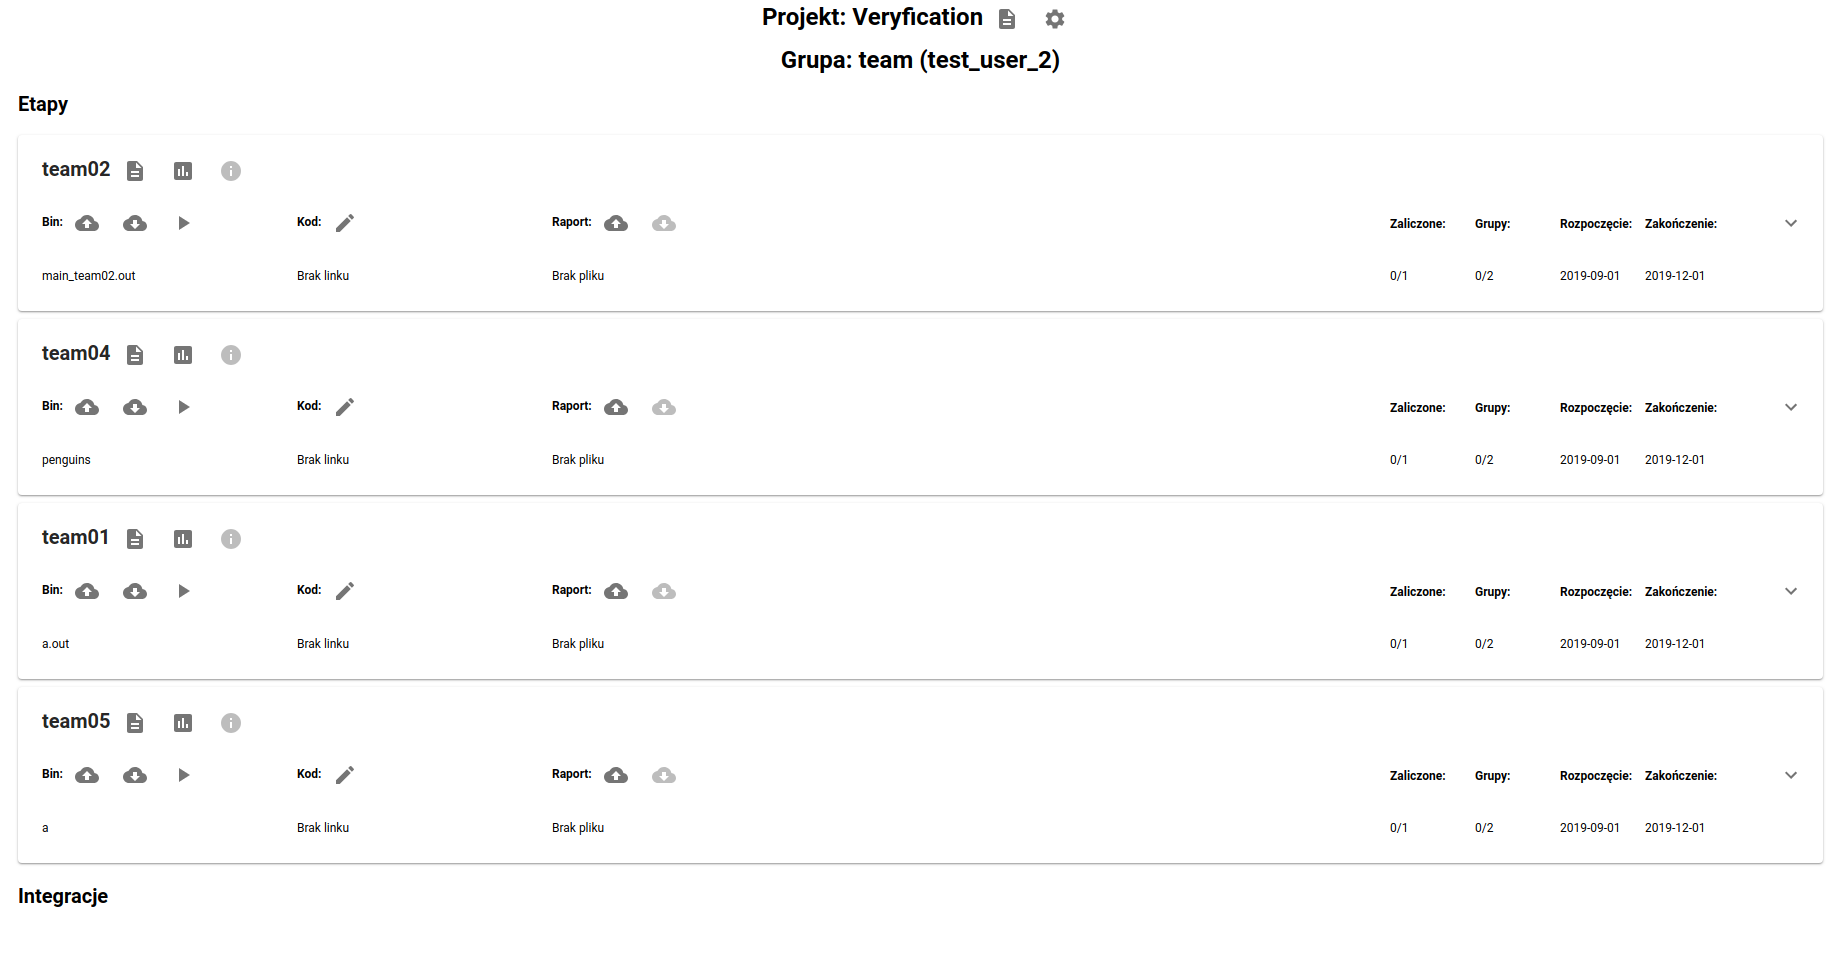
\includegraphics[width = 12cm]{chapter06/veryfication_first_project.png}
    \caption{Projekt dla weryfikacji platformy przy pomocy historycznych programów studentów (źródło własne).}
    \label{fig:veryfication_first_project}
\end{figure}

Dla każdego z czterech etapów (reprezentujących historyczne programy studentów) utworzono prosty przypadek testowy, gdzie jako \textit{input} i \textit{output} wprowadzono plik z planszą.
Został on wybrany losowo spośród zawartych w repozytoriach historycznych grup testowych plików wejściowych.
Następnie uruchomiono wszystkie cztery etapy.
Po przejrzeniu logów okazało się, że tylko jeden program uruchomił się poprawnie (załączony dla etapu \textit{team05}).
Była to aplikacja z tego samego repozytorium, z którego załączono plik z planszą do testów.
Inne dwa programy (etapy \textit{team02} oraz \textit{team04}) nie wypisały logów, natomiast jeden wypisał komunikat o niepoprawnym formacie pliku wejściowego (\textit{team01}).

Dla programu dołączonego do etapu \textit{team01} zmieniono plik wejściowy i wejściowy na takie, które znajdowały się w repozytorium razem z tym programem.
Aplikacja została następnie uruchomiona i wyniku swojego działania wypisała logi.

Programy załączone do etapów \textit{team02} oraz \textit{team04} zostały ponownie przeanalizowane poprzez lokalne uruchomienie.
W wyniku tego okazało się, że uruchamiają się one w wersji interaktywnej bez podawania argumentów wykonania.
Aby uzyskać informację zwrotną z ich działania utworzono nowy projekt z poniższą definicją środowiska:

{\fontfamily{qcr}\selectfont
\tiny
\begin{lstlisting}

    FROM gcc:4.9

    CMD ["./home/app"]

\end{lstlisting}
}

W ramach projektu zostały utworzone dwa etapy:  \textit{team02} oraz \textit{team04}.
Następnie załączono i uruchomiono programy.
Program załączony do etapu \textit{team02} uruchomił się w wersji interaktywnej i wypisał logi.

Aplikacja dla etapu \textit{team04} po raz kolejny nie zostawiła informacji zwrotnej z wyniku wywołania.
W celu rozwiązania problemu przeanalizowano część kodu aplikacji.
Ustalono, że problem może wynikać z pętli \textit{while}, która czeka na pobranie znaku od użytkownika.
Po usunięciu jej z kodu programu, rekompilacji i ponownym uruchomieniu programu na platformie uzyskano logi z wykonania aplikacji.


\section{Podsumowanie}
\label{verification_summary}

Wszystkie lokalnie uruchomione  historyczne programy  studenckie udało się uruchomić na platformie uzyskując przy tym informację zwrotną w postaci logów.
Jak łatwo zauważyć, taki sposób przetestowania programów nie przynosi wiele korzyści.
Równocześnie pokazuje na jak wiele problemów może napotkać prowadzący podczas procesu weryfkacji pracy studentów i w jak dużym stopniu wymaga on obecnie indywidualnego podejścia do każdej z grup.
Opisane w rozdziale komplikacje mogą wystąpić podczas sprawdzania każdego z etapów i nałożyć się w momencie próby przeprowadzenia integracji programów.

Jednak przy niewielkiej modyfikacji zadania, można osiągnąć dużo lepszą automatyzację procesu oceny efektów pracy zespołów.
W kolejnym rozdziale zostaną omówione zmiany założeń zadania historycznego, tak aby osiągnąć korzyści wynikające z korzystania z platformy.
Opisane również zostaną wnioski z przeprowadzenia symulacji zmodyfikowanego projektu historycznego na testowej grupie absolwentów.

TODO: dopisać w podsumowania:
- nie można ocenić poprawności działania projektów bez analizy kodu

- nie wiadomo co tam działa a co nie i jak

- integracja jest praktycznie nie możliwa bo programy przyjmują różne formaty planszy pomimo zdefiniowanego w założeniach zadania spójnego formatu

- prowadzący ma bardzo trudne zadanie

- ja z perspektywy czasu nie jestem w stanie ocenić poprawności programów

- trzeba mieć obok studentów żeby zrozumieć o co chodzi

- pomimo że wszyscy mieli te same założenia projektowe wynik końcowy to zupełnie różne projekty które nie mogą ze sobą współgrać

- studenci nawet w obrębie jednego projektu nie mają wypracowanego wspólnego protokołu

- to wszystko pokazuje, że platforma jest potrzebna



